\chapter{The Privacy monitoring system}
\label{pivot}
In this chapter, we introduce a Privacy-Monitoring system for LoRaWAN, named PIVOT. In Section \ref{goals}, we explain the main requirements to satisfy in developing our system, and in Section \ref{system} we describe PIVOT in detail, going from the assumptions adopted to its core algorithm and the metrics used.

\section{Design Goals}
\label{goals}
The following are the main points followed for the development of PIVOT.
\begin{enumerate}
	\item \textit{Strengthening} of the network.Our system should represent an additional security layer for the LoRaWAN protocol that can better preserve the confidentiality of the LoRa traffic exchanged between the endpoints and the Network Server 
	\item \textit{Detection} of vulnerable devices. Keeping in mind the threat described in Section \ref{address_identification},  PIVOT should identify the endpoints to which addresses could be linked by unauthorized listeners.
	\item \textit{Monitoring} the status of end-device. Our system should give the network operator a transparent vision of the state of the network, displaying the number of detected devices. 
	\item \textit{Modelling} the behavior of periodic devices. PIVOT should recognize the EDs that sends packets regularly and model their respective pattern.
	\item \textit{Minimize} the delay. Vulnerable devices need to be detected quickly to leave them exposed as little time as possible.
	\item \textit{Accuracy} of the detection. The detection procedure of PIVOT should be detailed and precise as far as possible. The error rate should be kept low.
	\item \textit{Easy and Lightweight}. The system should be designed to have a small memory footprint (RAM usage) and low CPU usage, overall a low usage of system resources.
	\item \textit{Passivity} of the system. Our engine should collect and analyzes uplink LoRa packets without interfering with the normal operations of the network.
	\item \textit{Scalability}. Our program should be able to scale, working well on both a small data set and a larger one.
\end{enumerate}

\section{System Description}
\label{system}
% detection procedure
The main policy of our system is to detect and protect devices in the LoRa network that are vulnerable to information disclosure. Going into detail, PIVOT passively collects and analyzes LoRa RF messages. When it discovers an uplink frame sent from a device with a DevAddress \(\ a \) it has never seen, checks which of the following two circumstances is met:
\begin{enumerate}
	\item The DevAddress \(\ a \) is linked to an ED that joins the network for the first time.
	\item The DevAddress \(\ a \) is linked to an ED already in the network that has disconnected and performed a new join procedure.
\end{enumerate}
In the case of the second scenario, PIVOT recognizes the weakness of the ED and it notifies the operator, that had to modify the parameters of the device to prevent it from being identified again.

\vspace{5mm} %5mm vertical space

% monitoring procedure
In addition, PIVOT supports the network operator in optimization operations. By monitoring the traffic, it computes a set of statistical metrics that display to the administrator the actual state of the network, reporting the current number of join/re-joined devices and correlated percentage of vulnerable endpoints that are still operating. In this way, the operator can check the level of security of the network and, if needed, execute actions to lower the level of exposed EDs.

\vspace{5mm} %5mm vertical space

% architecture
\begin{figure}[H]
    \centering
    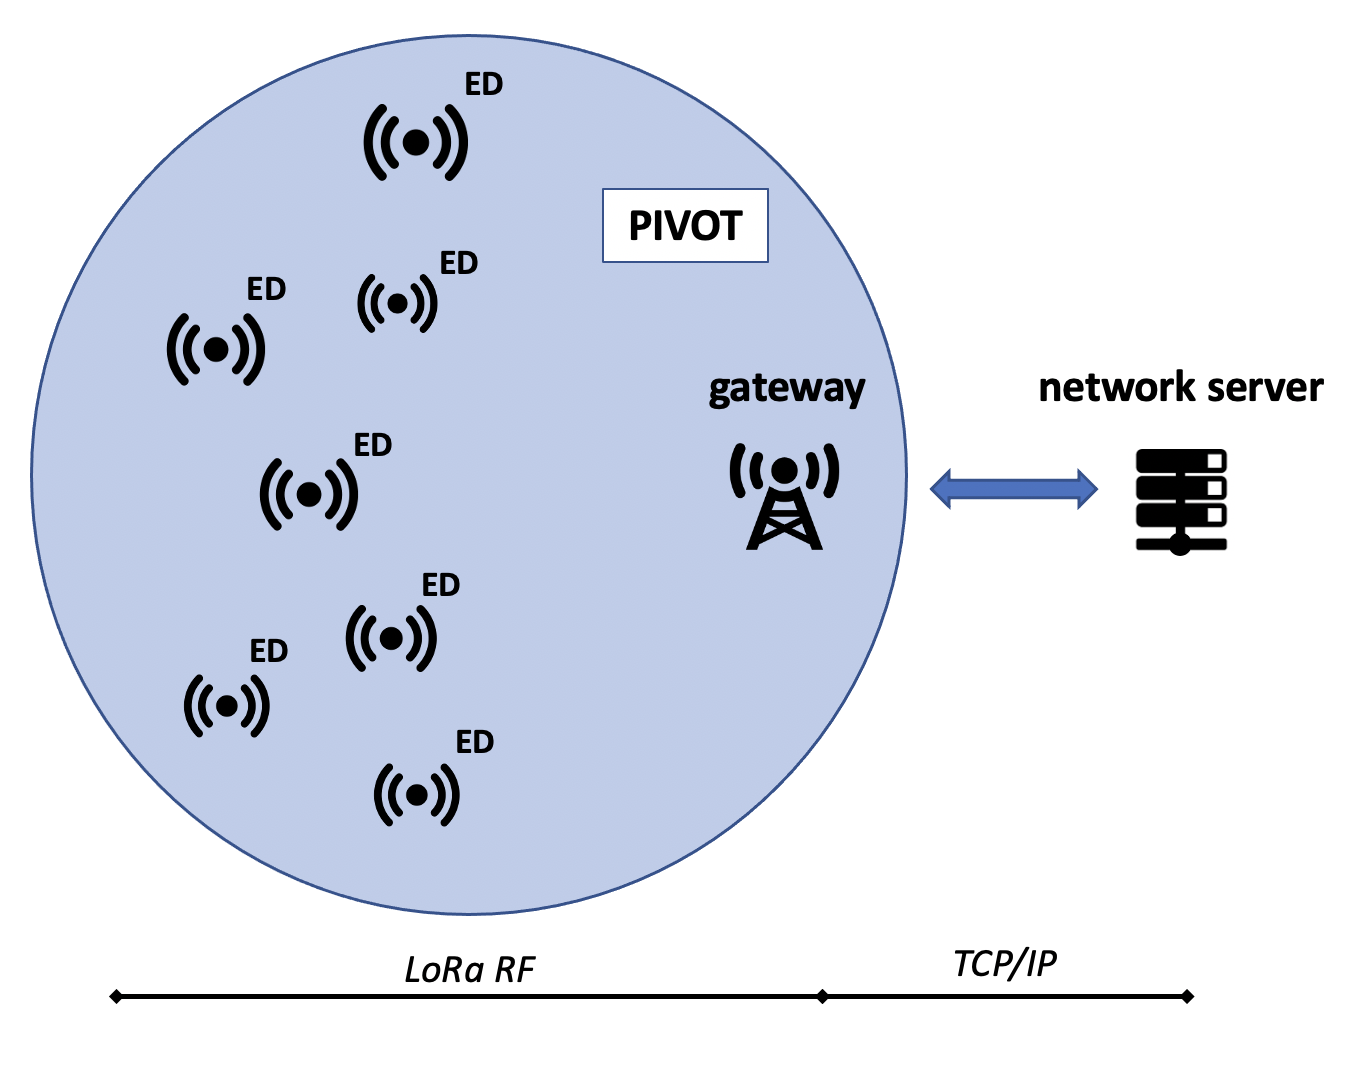
\includegraphics[width=0.7\linewidth]{images/pivot/architecture.png}
    \caption{The coverage area of PIVOT}
    \label{fig:piv_architecture}
\end{figure}
As shown in Figure \ref{fig:piv_architecture}, our system eavesdrops on the whole LoRa radio link area, filtering only \textit{uplink} LoRa packets that endpoints send to the Network Server. Since symmetric key encryption is applied only to the payload, PIVOT has complete access to the text-clear header of the frames it collects. In particular, it requires the fields reported in Table \ref{tab:keys}.
\begin{table}[h!]
    \caption{Key fields in the header, used by PIVOT}
    \label{tab:keys}
    \centering
    \begin{tabular}{|l|l|}
    \hline
        \textbf{PARAMETER} & \textbf{DESCRIPTION}                       \\ \hline
        DEV\_ADDR          & Unique identifier of the ED in the network \\ \hline
        DEV\_EUI           & Unique identifier of the physical ED       \\ \hline
	    FCnt		       & Frame counter                              \\ \hline
        TMST               & Internal clock timestamp                   \\ \hline
        TYPE               & Type of packet                             \\ \hline
    \end{tabular}
\end{table}

\subsection{Assumptions}
We assume that PIVOT passively monitors the LoRa RF traffic, filtering only \textit{uplink} and \jr packets sent by EDs to the gateway. The endpoints of the LoRa network in which PIVOT operates should be LoRaWAN v1.1 compliant and keep the same DevAddress for the entire connection. When they disconnect or lose the connection with the Network Server, they should try a new activation procedure, which gives them the new DevAddress. We require that devices perform exclusively the Over-the-Air Activation (OTAA) to join the network so that PIVOT can intercept \jr messages with a DevEUI exposed in the header as part of the activation procedure.
\\
Another assumption is that these devices should transmit packets periodically. These conditions find evidence in real case studies. For example, the analysis carried out on a LoRaWAN service of an Italian operator \cite{devil} shows up that the majority of devices send 24 packets each hour, the 25th one after 30 seconds, and then repeat the process. In other words, when a device sends uplink packets periodically, it follows a temporal pattern that repeats continuously over time with a period \(\tau\).

\subsection{Patterns}
In other words, when a device sends uplink packets periodically, it follows a temporal pattern that repeats continuously over time with a period \(\tau\). PIVOT focuses on the time elapsed between an uplink message and the next one from the same endpoint.
\begin{figure}
    \centering
    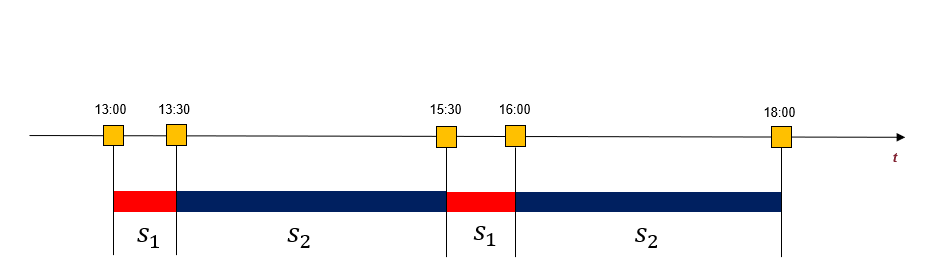
\includegraphics[width=0.7\linewidth]{images/pivot/pattern.PNG}
    \caption{An example of pattern \(\ P \)}
    \label{fig:pattern}
\end{figure}
In detail, let \(t_{i}\) the timestamp (TMST) of a packet \(p\) with a frame counter (FCnt) \(p_{fcnt} = i\), we define the segment \(\ s_{i} \):
\[\ s_{i} = t_{i+1} - t_{i} \]
as the temporal distance between two consecutive messages with the same DevAddress (DEV\_ADDR) and the pattern \(\ P \) with period \(\tau\) as a chain of segments: 
\[\ P_{a} = \{ s_{1}, s_{2}, ... \}\]
Clearly, \(\ \tau = s_{1} + ... + s_{n} \) where \(\ n \) is the number of segments in the chain of \(\ P \). For example, a device that sends packets each hour, has a pattern \(\ P = \{s\} \), with \(\ s = 1.0 \).
\\
PIVOT keeps track of every initialized pattern \(\ P \) by storing the following data:
\begin{itemize}
	\item The chain of segment \(\ \{ s_{1}, ..., s_{n} \} \) that composes the pattern \(\ P \).
	\item The current DevAddress \(\ a \) of the device.
	\item The timestamp \(\ t_{f} \) of the last packet sent by the device.
	\item A flag \textit{verified}, set to True if the pattern is complete.
\end{itemize}

\subsubsection{Update patterns}
When arrives a packet \(\ p \) with DevAddress \(\ a \) and timestamp \(\ t \), PIVOT calls the function \textit{updatePattern(a, t)}, that calculates the segment \(\ s = t - t_{f} \) and compares it with the chain of \(\ P \). 
If \(\ s \notin P \), the chain of the pattern \(\ P \) is not yet complete: the function appends this segment at the bottom of the chain \(\ P \gets s \) and sets the flag \(\ verified = False \).

\vspace{5mm} %5mm vertical space

\subsubsection{Pattern matching}
PIVOT labels different patterns as necessarily linked to separate devices. It classifies two patterns \(\ P_{1} \) and \(\ P_{2} \) as distinct if:
\begin{enumerate}
	\item Their chains are composed of different segments. 
	\item Their chains are composed of the same segments distributed in a different order.
	\item The first pattern's chain is a subset of the second pattern's chain.
\end{enumerate}
\begin{figure}
    \centering
    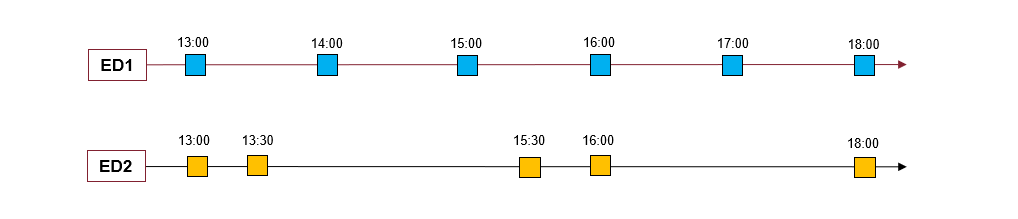
\includegraphics[width=0.7\linewidth]{images/pivot/patterns.PNG}
    \caption{}
    \label{fig:patterns}
\end{figure}
The first ED, which DevAddr \(\ a_{1} \), sends to the NS a packet each hour, the second one, which DevAddr is \(\ a_{2} \), sends a packet to the NS, waits 30 minutes, sends another packet, waits 2 hours, and repeats this sequence.  The first pattern consists of a single one-hour segment \(\ s_{1} = 1.0 \), the second one of two segments, one of 30 minutes \(\ s_{2} = 0.5 \) and one of 2 hours \(\ s_{3} = 2.0 \). In other words, given the following patterns: \(\ P_{1} = \{s_{1}\} \) with period \(\ \tau = 1.0 \) and \(\ P_{2} = \{s_{2}, s_{3}\} \) with period \(\ \tau = 2.5 \), Clearly, \(\ P_{1} \neq  P_{2} \) since their chains contains different segments. In the following section, we go deeper and analyze the algorithm used by PIVOT to identify vulnerable devices.

\subsection{Detection procedure}
PIVOT keeps track of all the devices it detects through a vector \(\ C \). It contains the tuples \(\ <a, P_{a}> \), where \(\ a \) is the current DevAddress of a ED, and \(\ P_{a} = \{ s_{1}, ..., s_{n} \} \) the pattern it follows. In \(\ C \), there cannot be two tuples that link to same device. If \(\ E \) the set of all the ED joined in the network, necessarily \(\ length(C) \subseteq length(E ) \). 
\\
If after a Join Request, PIVOT gets from a packet \(\ p \) a never-seen DevAddress \(\ a \), it verifies if that device is already in the network (then, it is in \(\ C \), represented by its old DevAddress), or is a new ED to add in \(\ C \). 


In other words, it compares the pattern \(\ P_{a} \), that is associated with the new DevAddress \(\ a \) to the patterns stored in \(\ C \). If there is a matching, \(\ a \) belongs a re-joined device.e
\\
The algorithm follows two sequential steps:
\begin{enumerate}
	\item Pre-Join procedure.
	\item Main procedure.
\end{enumerate}

\begin{figure}
    \centering
    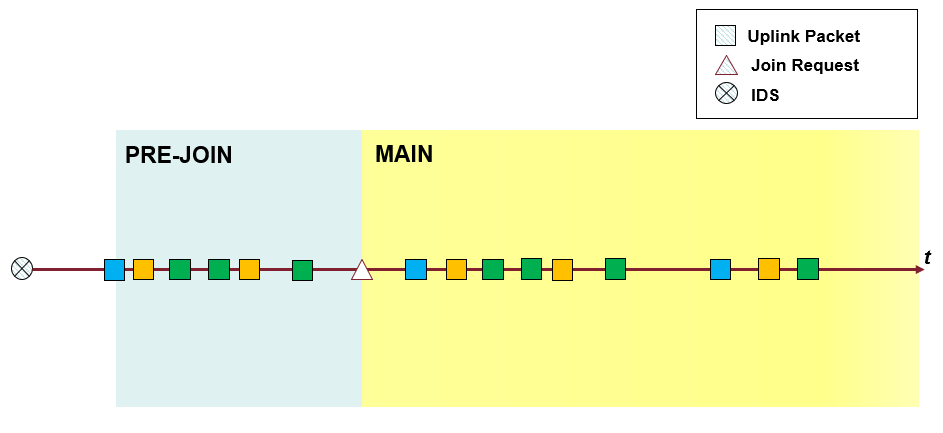
\includegraphics[width=0.7\linewidth]{images/pivot/pre-main.PNG}
    \caption{Graphical representation of the Pre-Join and Main procedures}
    \label{fig:pre_main}
\end{figure}

Let \(\ t_{0} \) the timestamp of the first packet received by PIVOT after its activation and \(\ t_{f} \) the timestamp of the first Join Request packet. The Pre-Join procedure has a limited duration and takes place in the time window \(\ t_{f} - t_{0} \). The Main procedure starts after the reception of the first Join-Request message, at \(\ t_{f} \) and remains active indefinitely.


\subsubsection{Pre-Join procedure}
The Pre-Join procedure gives to PIVOT an initial view about which EDs are currently operating in the network. Indeed, when the first packet \(\ p \) with timestamp \(\ t_{0} \) arrives, PIVOT has no historical trace of other devices in the network, either of the messages they sent. In other words, the vector \(\ C \) is empty.
\\
PIVOT, for each DevAddress \(\ a \) received in input:
\begin{itemize}
	\item If \(\ a \notin  C\), it initializes an empty pattern \(\ P = \{\} \) and inserts the tuple \(\ <a, P_{a} > \) in \(\ C \).
	\item If \(\ a \in C\), it updates the pattern \(\ P_{a} \gets C \).
\end{itemize}
The Pre-Join terminates when intercepts a \texttt{Join request} message for the first time. In this way, the number of DevAddress \(\ a_{1}, a_{2}, ..., a_{n} \) collected during this phase matches with the number of devices that sent messages \(\ ED_{1}, ED_{2}, ..., ED_{n} \). Indeed, in LoRaWAN, an \(\ ED_{i} \) modifieds its DevAddress \(\ a_{i} \) only when it disconnects from the network and performs an OOTA again. Since the Pre-Join procedure ends at \(\ t_{f} \) (where the first Join Request arrives), there cannot be any \(\ ED \) changing the associated Dev Addresses in the time-frame \(\ t_{f} - t_{0} \).

\begin{algorithm}
    \caption{Pre-Join procedure}
    \begin{algorithmic}[1]
        \If{$a$ in $C$}
            \State $P \gets C(a)$
            \State $P.update(t)$
        \Else
            \State $P \gets newPattern(a)$
            \State $C(a) \gets P$
        \EndIf
    \end{algorithmic}
\end{algorithm}

At the end of this task, the list \(\ C \) is filled with unique tuples \(\ <a, P_{a}> \). Nevertheless, some patterns may be incomplete. The time-frame \(\ t_{f} - t_{0} \)may be too small to estimate correctly the period \(\ \tau\) of all the patterns. Let's do an example:
There are two devices, ED1 and ED2, with two different patterns \(\ P_{1} = \{ s_{1} \} \) and \(\ P_{2} = \{ s_{2}, s_{3} \} \), where \(\ s_{1} = 0.5 \), \(\ s_{2} = 0.33 \) and \(\ s_{3} = 2.0 \). If the Pre-Join has a time frame \(\ t_{f} - t_{0} = 1.75 \), the algorithm can't determine \(\ P_{2} \). On the contrary, since ED1 sends packets following a smaller period \(\ \tau = 0.5\), PIVOT recognizes correctly \(\ P_{1} \).
\begin{figure}
    \centering
    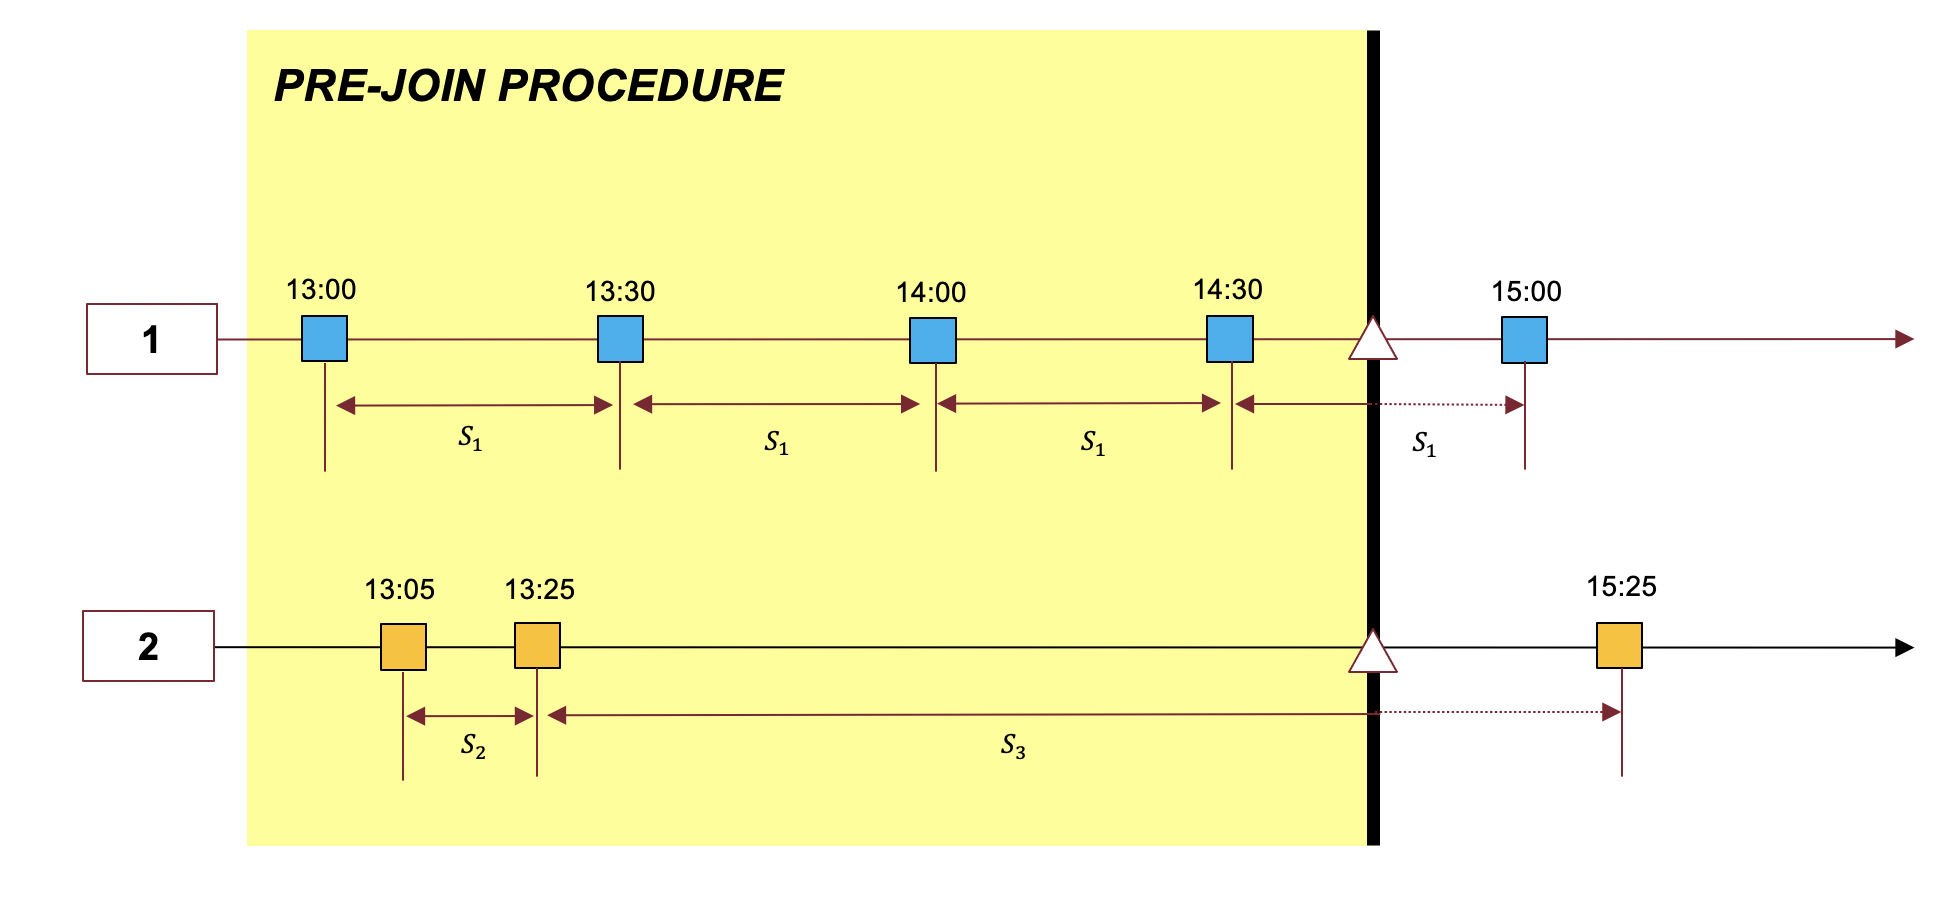
\includegraphics[width=0.7\linewidth]{images/pivot/missing_pattern.png}
    \caption{}
\end{figure}

PIVOT label as \texttt{verified} all the DevAddress \(\ a \) with a complete pattern \(\ P \) (such as \(\ P_{1} \) in the previous example). If define \(\ V \) as the list of verified patterns \(\ V \gets verified(C) \), then \(\ V \subseteq C\).

\subsubsection{Main procedure}
Unlike the previous stage, PIVOT cannot guarantee that a never-seen DevAddress \(\ a \) necessarily belongs to a new device. For each packet \(\ p \) received as input, we can have:
\begin{itemize}
	\item The DevAddress \(\ a \) is associated with a confirmed pattern \(\ P_{a} \) of \(\ C \). Then \(\ a \) belongs to an old ED already registered in the Pre-Join procedure.
	\item The DevAddress \(\ a \) is unknown. We cannot establish if it belongs to a new device or an old one that re-joined the network.
\end{itemize}

\begin{algorithm}
    \caption{Main procedure}
    \begin{algorithmic}[1]
        \If{$a$ not in $C$}
            \If{$a$ in $U$}
                \If{$a$ in $Q$}
                    \State quarantine procedure
                \EndIf
                \State $V \gets verified(A)$
                \ForAll{$v$ in $V$}
                    \If{$match(P_{a}, P_{v})$}
                        \State $Q \gets a$
                    \Else
                        \State $A(a).remove(P_{v})$
                    \EndIf
                \EndFor
                \If{$A(a)$ is empty}
                    \State new device
                    \State $C \gets P_{a}$
                \EndIf
            \Else
                \State $P \gets newPattern(a)$
                \State $U(a) \gets P$
                \State $A(a) \gets C$
            \EndIf
        \EndIf
    \end{algorithmic}
\end{algorithm}

In the second scenario, PIVOT initialize a pattern \(\ P_{a} \) and puts it in the unconfirmed list \(\ U \). Then it compares \(\ P_{a} \) to the verified patterns of \(\ V \gets verified(C) \). If \(\ P_{a} \) doesn't match any element of \(\ C \), then PIVOT conclude it is unique and that the DevAddress \(\ a \) necessarily represents a new ED. PIVOT updates the \(\ C \) appending this new pattern \(\ C \gets P_{a} \). Otherwise, if there is a match \(\ P_{a} \equiv P_{v}\), PIVOT puts \(\ a \) in a new list we called Quarantine \(\ Q\). In detail, two patterns \(\ P_{1} = \{ s_{1}, ..., s_{n} \}\) and \(\ P_{2} = \{ s_{1}, ..., s_{n} \}\) matches when their segments are of the same lenght and follows the same sequence.
% formula
% aggiornamento dei segmenti
When PIVOT recevis a packet \(\ p \) with DevAddress \(\ a \) and timestamp \(\ t \), it calculates the segment \(\ s = t - t_{a} \), where \(\ t_{a} \) is the last timestamp, and updates the pattern \(\ P_{a} \). For example, given a scenario where to the DevAddress \(\ a \) is linked a incomplete pattern \(\ P_{a} = \{ s_{1}, s_{2} \}\) where \(\ s_{1} = 0.5 \) and \(\ s_{2} = 2 \). If \(\ s = t - t_{a} = 0.5 \), PIVOT labels \(\ P_{a} \) as complete and expects that the next \(\ s = t - t_{a} \) will be 2.

\subsubsection{Quarantine}
\begin{figure}[t]
    \centering
    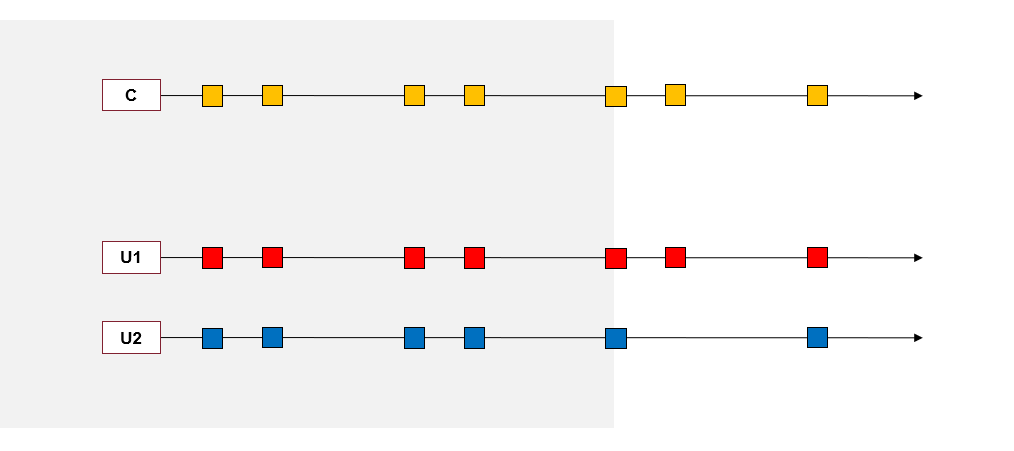
\includegraphics[width=0.7\linewidth]{images/pivot/quarantine.PNG}
    \caption{Quarantine}
    \label{fig:quarantine}
\end{figure}
When the incoming packet \(\ p \) has a DevAddress \(\ a \in Q \), it means that the linked pattern \(\ P_{a} \) matches exactly with a pattern P of the \(\ C \) list. We can have two scenarios:
\begin{enumerate}
	\item \(\ P_{a} \) and \(\ P \) belongs to the same ED.
	\item  \(\ P \) and \(\ P_{a} \) are linked to different ED but \(\ P \subseteq P_{a} \).
\end{enumerate}
Given the timestamp \(\ t \) of the current packet \(\ p \), PIVOT calculates the segment \(\ s = t - t_{a} \), updates \(\ P_{a} \) and check if \(\ P \) and \(\ P_{a} \) still match. If so, PIVOT updates the DevAddress linked to \(\ P \) with \(\ a \) and warns the operator. If not, \(\ P_{a} \) belongs to a new deive, then moves from \(\ U \) to \(\ C \).
\begin{algorithm}[h!]
    \caption{Quarantine}
    \begin{algorithmic}[1]
        \If{$a$ in $C$}
            \State $P \gets C(a)$
            \State $P.update(t)$
        \Else
            \State $P \gets newPattern(a)$
            \State $C(a) \gets P$
        \EndIf
    \end{algorithmic}
\end{algorithm}

\subsection{Monitoring procedure}
In this section, we first describe the metrics used by PIVOT to enumerate the percentage of identified weak devices in the network. Then, we explain how the operator can use these metrics to evaluate the effectiveness of the countermeasures it applies.